

\section{Intro to HTML (\& Bootstrap)}

\begin{frame}{Understanding websites\dots}
    \metroset{block=fill}
    Why are we doing this workshop? The motivation from our abstract:
    \begin{itemize}
        \item[\textcolor{w3schools}{\faCheck}] But what happens after an edition is encoded in TEI? 
        \item[\textcolor{w3schools}{\faHandORight}] While it is an \textbf{ideal format for archiving digital data}, it is \alert{less than ideal for viewing and interacting with the edited text.}
        \item[\textcolor{w3schools}{\faHandORight}] The data transformation language XSLT allows editors to create multiple representations from their data encoded in XML, enabling the creation of both digital and print editions. 
    \end{itemize}
    
    \begin{block}{Goals for the next session}
    \begin{enumerate}
        \item[\textcolor{w3schools}{\faCheck}] learn some theory basics
        \item[\textcolor{w3schools}{\faCheck}] everybody on the same page on XML/TEI for digital editing
        \item[\textcolor{alert}{\faClose}] creating websites in HTML (\& Bootstrap)
    \end{enumerate}
    \end{block}
\end{frame}

%-----------------------------------------------------


\begin{frame}[fragile,allowframebreaks]{Hyper Text Markup Language (HTML)}
\metroset{block=fill}\small 

\begin{columns}
\column{0.4\textwidth}
\bgupper{w3schools}{black}{.html}\\
Defines the structure of websites. Due to their common origin in SGML: lots of similarity with XML but, unlike XML's extensibility, HTML has a fixed tag set (much less!). 


\begin{block}{The most important HTML elements to remember }
html, head, body.
div, p, h1-6.
span,
ul, ol, li.
table, tr, td.
\end{block}

\column{0.58\textwidth}
\begin{htmlcode}
<!DOCTYPE html>
<html>
 <head>
  <title>Page Title</title>
  <style> /* preferably in extra file */
   p.important {
    color: green;
    }
  </style>
  <script>
    alert("Hello! I am an alert box!!");
  </script>
 </head>
 <body>
  <h1>This is a Heading</h1>
  <p style="color:red">I am a paragraph</p>
  <p>I like
   <span style="color:blue">blue</span>.</p>
  <p class="important">
   Note that this important!</p>
  </body>
</html>
\end{htmlcode}
(full example on the next slide)
\end{columns}

\framebreak

\begin{columns}
\column{0.4\textwidth}
\begin{htmlcode}
<!DOCTYPE html>
<html>
 <head>
  <title>Page Title</title>
  <style> /* better in extra file */
  h1 {
   color: blue;
   font-family: verdana;
   font-size: 300%;
   }
   p  {
    color: red;
    font-family: courier;
    font-size: 160%;
    }
   p.important {
    color: green;
    }
  </style>
  <script>
    alert("Hello World!");
   </script>
 </head>
\end{htmlcode}

\column{0.58\textwidth}
\begin{htmlcode}
 <body>
  <h1>This is a Heading</h1>
  <p>This is a paragraph. <br />
    <a href="https://www.w3schools.com">
    This is a link</a>
  </p>
  <img src="img.jpg" 
    width="500" height="600" />
  <p style="color:red">I am a paragraph</p>
  <p title="I'm a tooltip">
    This is a paragraph.
  </p>
  <p>My mother has 
     <span style="color:blue">blue</span>
     eyes.</p>
  <p class="important">
    Note that this is an important 
    paragraph. :)</p>
 </body>
</html>
\end{htmlcode}
\end{columns}

\end{frame}

%--------------------------------------------------
\begin{frame}[fragile]{CSS}
\footnotesize
\metroset{block=fill}
\begin{columns}
\column{0.48\textwidth}
\bg{alert}{white}{CSS = Cascading Style Sheets}\\
\bgupper{w3schools}{black}{.css}\\
\begin{block}{}
\begin{itemize}
    \item included via a stylesheet link in HTML or written inline
    \item describes the styling of websites 
    \item separation of form \& content: 
    \begin{itemize}\scriptsize
        \item \textbf{HTML:} content in structured form
        \item \textbf{CSS:} the layout
        \item (\textbf{JavaScript:} dynamic parts)
    \end{itemize}
    \item the \bg{w3schools}{white}{\href{http://getbootstrap.com/}{Bootstrap framework}} offers a ready-made, responsive design to reuse: box and grid model
    \item uses selectors to define layout
\end{itemize}
\end{block}

\begin{csscode}
h1 {
font-family: Arial
}
\end{csscode}


\column{0.48\textwidth}
\begin{csscode}
p {
font-family: Arial ;
color: red
}
\end{csscode}

\begin{csscode}
.person {
    font-weight:bold;
    font-size:smaller;
    font-style:italic;
}
\end{csscode}

\begin{block}{Resources}
\begin{itemize}\scriptsize
    \item \href{https://tutorialzine.com/2015/10/learn-the-bootstrap-grid-in-15-minutes}{15min to Bootstrap}
    \item \href{http://www.smashingmagazine.com/wp-content/uploads/images/css3-cheat-sheet/css3-cheat-sheet.pdf}{CSS3-Cheatsheet}
    \item \textbf{W3 Schools:} \href{http://www.w3schools.com/css/}{W3schools CSS} 
    \item \href{http://www.w3.org/TR/CSS21/propidx.html}{W3S Tables of properties}
    \item \href{http://www.csszengarden.com}{CSS ZenGarden}
\end{itemize}
\end{block}

\end{columns}

\end{frame}

%--------------------------------
\begin{frame}[fragile]{JavaScript}
\metroset{block=fill}
\bg{alert}{white}{modifying websites dynamically}\\
\bgupper{w3schools}{black}{.js}\\
\begin{itemize}\small 
    \item JS can change websites without having to reload them (`dynamically'). {\scriptsize remember when you had to manually refresh pages?}
    \item When we want to highlight something using a check box, we use js. 
    \item Unlike HTMl (which is a markup language, think of it like a file format), js is a programming language (like XSLT).
    \item \alert{$\to$ we won't learn this today!} {\footnotesize But there is a mini example and you will load js components when using Bootstrap and the GAMS wippets later.}
\end{itemize}


\begin{block}{A `Hello World!' example}
\begin{jscode}
document.getElementById("demo").innerHTML = "Hello JavaScript";
\end{jscode}
\end{block}

\end{frame}


%--------------------------------------------------

\begin{frame}[fragile, allowframebreaks]{Bootstrap Framework}
\metroset{block=fill}\footnotesize 
\begin{block}{}
\begin{quote}
    Bootstrap is a free and \textbf{open-source CSS framework} directed at \textbf{responsive, mobile-first front-end web development.} It contains HTML, CSS and (optionally) JavaScript-based design templates for typography, forms, buttons, navigation, and other interface components. (\href{https://en.wikipedia.org/wiki/Bootstrap_(front-end_framework)}{Wikipedia})
\end{quote}
\end{block}

\begin{block}{How to use Bootstrap?}
\begin{enumerate}
    \item load the scripts in the HTML head
    \item figure out new \href{https://getbootstrap.com/}{Bootstrap} elements using \href{https://www.w3schools.com/bootstrap/}{W3Schools Tutorials}.
    \begin{itemize}\scriptsize
        \item \protect\url{https://www.w3schools.com/howto/}
        \item \protect\url{https://www.w3schools.com/bootstrap/}
    \end{itemize}
\end{enumerate}
\end{block}

\framebreak 

We need to include the bootstrap stylesheet from this  \href{https://getbootstrap.com/docs/4.0/getting-started/introduction/}{<link>} in the HTML  \texttt{<head>} but also the javascript plugins. 

\begin{block}{}
Careful, \texttt{<head>} in HTML is equivalent to the \texttt{<teiHeader>}. Headings in HTML are called: \texttt{<h1>-<h6>}.
\end{block}
Under \href{https://getbootstrap.com/docs/4.0/examples/}{<examples>}, Bootstrap offers different types of ready-to-use websites. I have included one in our practice XSL templates. {\scriptsize  $\to$ \href{view-source:https://getbootstrap.com/docs/4.0/examples/starter-template/}{Link to the source-Code of the starter template} $\to$ append it in the address or click right and `inspect element' or sth)}

\begin{htmlcode}
<html>
    <head>
    <meta charset="utf-8">
    <link rel="stylesheet" href="https://...bootstrap.min.css">
    <script src="https://code.jquery.com/jquery-3.2.1.slim.min.js"></script>
    </head>
    <body> [...] </body>
</html>
\end{htmlcode}


\framebreak 

\begin{htmlcode}
<!doctype html>
<html lang="en">
  <head>
    <!-- Required meta tags -->
    <meta charset="utf-8">
    <meta name="viewport" content="width=device-width, initial-scale=1">

    <!-- Bootstrap CSS -->
    <link href="https://cdn.jsdelivr.net/npm/bootstrap@5.1.3/dist/css/
    bootstrap.min.css" rel="stylesheet"
    integrity="sha384-1BmE4kWBq78iYhFldvKuhfTAU6auU8tT94WrHftjDbr
    CEXSU1oBoqyl2QvZ6jIW3" crossorigin="anonymous">

    <title>Hello, world!</title>
  </head>
  <body>
    <h1>Hello, world!</h1>
    <script src="https://cdn.jsdelivr.net/npm/bootstrap@5.1.3/dist/
    js/bootstrap.bundle.min.js" 
    integrity="sha384-ka7Sk0Gln4gmtz2MlQnikT1wXgYsOg+
    OMhuP+IlRH9sENBO0LRn5q+8nbTov4+1p" 
    crossorigin="anonymous"></script>

  </body>
</html>
\end{htmlcode}

\end{frame}


%--------------------------------------------------
\begin{frame}{Resources}
\small\metroset{block=fill}
\begin{enumerate}
    \item \href{https://dash.generalassemb.ly/projects}{Lessons 1 and the start of 2 on Dash (signup required)}. 
    \item \href{https://www.codecademy.com/learn/learn-html}{Codecademy HTML} (good but verbos)
    \item Interneting is hard:
    \begin{itemize}\footnotesize
        \item \href{https://internetingishard.com/html-and-css/introduction/}{Intro} 
        \item \href{https://internetingishard.com/html-and-css/basic-web-pages/}{Chapter 2: HTML Basics}
    \end{itemize}
    \item \href{https://developer.mozilla.org/en-US/docs/Learn/HTML/Introduction_to_HTML/Getting_started}{Mozilla Learn HTML} \& \href{https://developer.mozilla.org/de/docs/Learn/HTML}{in German}
    \item \href{https://www.w3schools.com/html/exercise.asp}{W3Schools interactive HTML} or respectively the more text based \href{https://www.w3schools.com/html/default.asp}{HTML tutorial}. 
    \item \href{https://www.learn-html.org/en/Basic_Elements}{Learn HTML.org} 
    \item \href{https://jgthms.com/web-design-in-4-minutes/}{Web Design in 4 minutes (CSS)}
    \item \href{https://www.w3schools.com/html/html_responsive.asp}{W3Schools tutorials}
\end{enumerate}

\end{frame}


%--------------------------------------------------
\begin{frame}{\texttt{.html} files and your browser}
    \footnotesize\metroset{block=fill}
\begin{itemize}
    \item clicking on a \texttt{.html} file will open up a browser (which parses and interprets the code). This doesn't mean it's on the internet! (check the address line, it links to your local computer)
    \item ergo: the webbrowser's job is downloading a website's code, i.e. getting it for you, and also reading \& displaying that code. The second part is what happens when you open a local \texttt{.html} file.
    \item To inspect the code of a local file, open as text (for example in Oxygen XML).
    \item To inspect a web page's code online, right-click and chose `inspect' (or sth like that). In the Dev Tools, you can edit this code (only on your local browser, of course), try it out!
\end{itemize}

\begin{block}{}
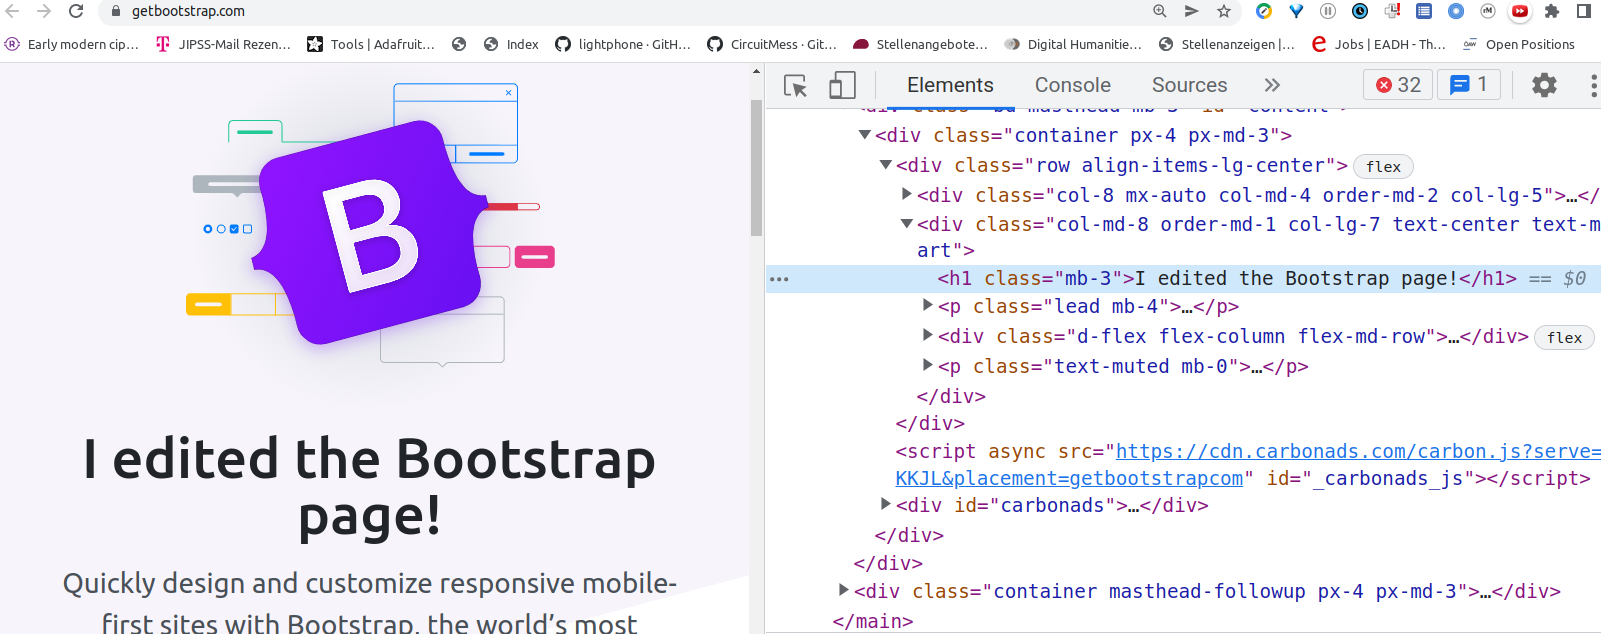
\includegraphics[width=0.9\textwidth]{img/bootstrap-dev-tools.png}
\end{block}

\end{frame}

%--------------------------------------------------


%------------------------------------------------------------------------------
\begin{frame}[standout]
    \alert{HTML Practice!} \\
    \normalsize
    To understand the basics of HTML and the `web triad' (HTML, CSS, JS) better, do one of the following exercises:
    \begin{enumerate}
        \item \alert{\href{https://dash.generalassemb.ly/}{`Dash' HTML / CSS tutorial}} (great but signup required)
        \item \alert{\href{https://www.w3schools.com/html/default.asp}{W3Schools tutorial}}
    \end{enumerate}
    
    Start working on the XPath/XSLT exercise sheet (resources/materials folder), XSLT 2.1 part. Feel free to use the slides and cheatsheet for help.
\end{frame}
